% v2-acmsmall-sample.tex, dated March 6 2012
% This is a sample file for ACM small trim journals
%
% Compilation using 'acmsmall.cls' - version 1.3 (March 2012), Aptara Inc.
% (c) 2010 Association for Computing Machinery (ACM)
%
% Questions/Suggestions/Feedback should be addressed to => "acmtexsupport@aptaracorp.com".
% Users can also go through the FAQs available on the journal's submission webpage.
%
% Steps to compile: latex, bibtex, latex latex
%
% For tracking purposes => this is v1.3 - March 2012

\documentclass[prodmode,acmtecs]{acmsmall} % Aptara syntax

% Package to generate and customize Algorithm as per ACM style
\usepackage[ruled]{algorithm2e}
\renewcommand{\algorithmcfname}{ALGORITHM}
\SetAlFnt{\small}
\SetAlCapFnt{\small}
\SetAlCapNameFnt{\small}
\SetAlCapHSkip{0pt}
\IncMargin{-\parindent}

% Metadata Information
\acmVolume{0}
\acmNumber{0}
\acmArticle{0}
\acmYear{2014}
\acmMonth{0}

% My own macros
\usepackage{epsfig}
\usepackage{listings}
\lstset{%
    language=C,
    basicstyle=\small\tt,
    numbers=left,
    numberstyle=\tiny
    }
\newcommand{\oh}[1]
    {\mbox{$ {\mathcal O}( #1 ) $}}
\newcommand{\eqn}[1]
    {(\ref{eqn:#1})}
\newcommand{\fig}[1]
    {Figure~\ref{fig:#1}}
\newcommand{\tabl}[1]
    {Table~\ref{tab:#1}}
\newcommand{\figs}[2]
    {Figures~\ref{fig:#1} and~\ref{fig:#2}}
\newcommand{\sect}[1]
    {Section~\ref{sec:#1}}
\newcommand{\cuda}
    {{\sc cuda}\xspace}
\newcommand{\namd}
    {{\sc namd}\xspace}
\newcommand{\acemd}
    {{\sc acemd}\xspace}
\newcommand{\fenzi}
    {{\sc fenzi}\xspace}
\newcommand{\mdcore}
    {{\tt mdcore}\xspace}
\newcommand{\swift}
    {{\sc swift}\xspace}
\newcommand{\bsf}[1]
    {\textbf{\textsf{#1}}}


% Document starts
\begin{document}

% Page heads
\markboth{P.~Gonnet}{QuickSched: Task-based parallelism with dependencies and conflicts}

% Title portion
\title{QuickSched: Task-based parallelism with dependencies and conflicts}
\author{PEDRO GONNET
\affil{Durham University}}
% NOTE! Affiliations placed here should be for the institution where the
%       BULK of the research was done. If the author has gone to a new
%       institution, before publication, the (above) affiliation should NOT be changed.
%       The authors 'current' address may be given in the "Author's addresses:" block (below).
%       So for example, Mr. Abdelzaher, the bulk of the research was done at UIUC, and he is
%       currently affiliated with NASA.

\begin{abstract}
Bla.
\end{abstract}

\category{???}{Computing methodologies}{Shared memory algorithms \and Concurrent algorithms}

\terms{Algorithms, Design, Performance}

\keywords{Task-based parallelism}

\acmformat{Pedro Gonnet, 2014.
QuickSched: Task-based parallelism with dependencies and conflicts.}
% At a minimum you need to supply the author names, year and a title.
% IMPORTANT:
% Full first names whenever they are known, surname last, followed by a period.
% In the case of two authors, 'and' is placed between them.
% In the case of three or more authors, the serial comma is used, that is, all author names
% except the last one but including the penultimate author's name are followed by a comma,
% and then 'and' is placed before the final author's name.
% If only first and middle initials are known, then each initial
% is followed by a period and they are separated by a space.
% The remaining information (journal title, volume, article number, date, etc.) is 'auto-generated'.

\begin{bottomstuff}
This work was supported by a Durham Universiy Seedcorn Grant.

Author's address: P. Gonnet, School of Engineering and Computing Sciences,
Durham University, South Road, Durham, DH1 3LE, United Kingdom.
\end{bottomstuff}

\maketitle


\section{Introduction}

Task-based parallelism is a conceptually simple paradigm for
shared-memory paralelism in which a computation is broken-down
into a set of inter-dependent tasks which are executed
concurrently.
Task dependencies are used to model the flow of data between
tasks, e.g.~if task $B$ requires some data generated by task $A$,
then task $B$ {\em depends} on task $A$ and cannot be executed
before task $A$ has completed.
The tasks and their dependencies can be seen as the nodes and edges
respectively of a Directed Acyclic Graph (DAG) which can be
traversed in topological order, executing the tasks at the nodes
on the way down.

This computational model is trival to parallelize.
Given a set of inter-dependent tasks and a set of computational
threads, each thread repeatedly selects a task with no
unsatisfied dependencies from the DAG and executes it.
If no tasks are available, the thread waits until any other
thread finishes executing a task, thus potentially releasing
new tasks, or until all tasks in the DAG have been executed.

\fig{Tasks} shows the DAG for a set of tasks.
The arrows indicate the direction of the dependency, i.e.~an
arrow from task $A$ to task $B$ indicates that task $B$ depends
on task $A$.
In a parallel setting, tasks $A$, $G$, and $J$ can be
executed concurrently.
Once task $G$ has completed, tasks $F$ and $H$ become available
and can be executed by any other computational thread.

\begin{figure}
    \centerline{\epsfig{file=figures/Tasks.pdf,width=0.5\textwidth}}
    \caption{A set of tasks (circles) and their dependencies (arrows).
        The arrows indicate the direction of the dependency, i.e.~an
        arrow from task $A$ to task $B$ indicates that task $B$ depends
        on task $A$.
        Tasks $A$, $G$, and $J$ have no unsatisifed dependencies and
        can therefore be executed.
        Once task $G$ has completed, tasks $F$ and $H$ become available.}
    \label{fig:Tasks}
\end{figure}

One of the first implementations of a task-based parallel programming
systems is Cilk \cite{ref:Blumofe1995}, an extension to the C
programming language which allows function calls to be ``spawned''
as new tasks.
Dependencies are enforced by the {\tt sync} keyword, which
forces a thread to wait for all the tasks that it spawned
to complete.
Although simple to use, this implicit dependency management
limits the types of DAGs that can be represented, i.e.~for
the example in \fig{Tasks}, using such a spawning model
would create implicit dependencies between the lowest-level
tasks $C$, $E$, and $K$.

In SMP superscalar \cite{ref:Perez2008}, StarPU \cite{ref:Augonnet2011},
QUARK \cite{ref:Yarkhan2011}, and KAAPI \cite{ref:Gautier2007}
the programmer spcifies
what shared data each task will access, and how that data will
be accessed, e.g.~read, write, or read-write access.
The dependencies between tasks are then generated
automatically by the runtime system, assuming that the
data must be accessed and updated in the order in which
the tasks are generated.
StarPU also provides an interface for specifying additional
dependencies explicitly.
Intel's Threding Building Blocks (TBB)
\cite{ref:Reinders2010}
provide task-based parallelism using C++ templates.
Dependencies are handled either by explicitly waiting
for spawned tasks, or by explicitly manipulating
task reference counters.

Finally, the very popular OpenMP standard provides some basic support
for spawning tasks, similar to Cilk, as of version 3.0
\cite{ref:OpenMP2008}.
OmpSs \cite{ref:Duran2011} extends this scheme with automatic
dependency generation as in SMP superscalar, along with
the ability to explicitly wait on certain tasks.

In all of these systems, the tasks are only aware of a single
type of relationship between each other, i.e. dependencies, which
specify a strict ordering between two tasks.
In many cases, however, the task ordering need not necessarily
be this strict.
Consider the case of two tasks that update some shared resource
in an order-independent way, e.g. when accumulating a result in
a shared variable, or exclusively writing to an output file.
In order to avoid concurrent access to that resource, it is
imperative that the execution of both tasks does not overlap,
yet the order in which the tasks are exectued does not matter.
In the following, such a relationship will be refered to
as a ``conflict'' between two tasks.
\fig{TaskConflicts} shows a task graph with conflicting tasks
joined by thick dashed lines.
None of tasks $F$, $H$, and $I$ cannot be executed concurrently,
i.e. they must be serialized, yet in no particular order.

Conflicts can be modeled as exclusive locks on a shared resource
which have to be obtained by a task before it can execute.
Thus, in \fig{TaskConflicts}, before executing, task $F$ has
to obtain an exclusive lock on the resource associated with
the conflict between tasks $F$, $H$, and $I$.
While task $F$ is being executed, neither $H$ nor $I$ can 
lock the same resource, and therefore will not execute until
task $F$ is done and the lock has been released.

In dependency-only systems, such conflicts can be modelled
with dependencies, which enforce a pre-determined arbitrary
ordering on conflicting tasks.
This, however, imposes unnecessary restriction on the order
in which tasks can be scheduled, especially in the presence
of multiple conflicts per task.
Both \citeN{ref:Ltaief2012} and \citeN{ref:Agullo2013} note
this problem in their respective implementations of the Fast Multipole
Method, in which forces computed in different tasks are
accumulated on a set of particles.

This paper presents QuickSched, a framework for task-based
parallel programming with constraints.
Section~2 describes the underlying algorithms and data structures,
and Section~3 describes their specific implementation in QuickSched.
Section~4 presents two test-cases:
\begin{itemize}
    \item The tiled QR
    decomposition described in \cite{ref:Buttari2009} and for
    which the QUARK scheduler was originally developed,
    \item A task-based Barnes-Hut tree-code to compute the
    gravitational N-body problem,
\end{itemize}
These real-world examples show how QuickSched can be used in practice,
and can be used to assess its efficiency.
Section~5 concludes with some general observations and future work.

\begin{figure}
    \centerline{\epsfig{file=figures/TaskConflicts.pdf,width=0.5\textwidth}}
    \caption{Task graph with conflicts (thick dashed lines).
        If two or more tasks are joined by a conflict, they cannot be
        executed concurrently, i.e. tasks $B$ and $D$ cannot be run an
        the same time.
        Tasks belonging to different conflicting sets, e.g. tasks $B$
        and $F$, or tasks $F$ and $J$, however, can be executed
        concurrently.}
    \label{fig:TaskConflicts}
\end{figure}


\section{Data Structures and Algorithms}

The QuickSched task scheduler consits of four main
objects types: {\em task}, {\em resource}, {\em scheduler},
and {\em queue}.

The task and resource objects are used
to model the computation, i.e. the work that is to be done
and the data on which it will be done, respectively.
The scheduler and queue objects manage
how the work is done, i.e. which tasks get scheduled
where and when, respectively.

\begin{figure}
    \centerline{\epsfig{file=figures/QSched.pdf,width=0.7\textwidth}}
    \caption{Schematic of the QuickSched task scheduler.
        The tasks (circles) are stored in the scheduler (left).
        Once a task's dependencies have been resolved, the task
        is moved to one of the task queues.
        Tasks that are not involved in any active conflicts
        are then taken from the queues by the different
        computational threads and executed.
        After execution, their dependent tasks are unlocked
        in the scheduler (dashed arrow).}
    \label{fig:QSched}
\end{figure}

The division of labour regarding {\em correctness}
between the scheduler and
the queue objects is illustrated in \fig{QSched}.
The scheduler holds the tasks and is in charge
of managing {\em dependencies}.
Once a task has no unresolved dependencies, it is passed
on to a queue object.
The queue object, on the other hand, is in charge
of managing {\em conflicts}.
Computational threads can query a queue and will
receive only tasks for which all conflicts have been
resolved, i.e. for which all necessary resources could be 
exclusively locked.

There is also a division of responsibilities regarding
{\em efficiency} between the scheduler and the queue
objects.
The tasks in each queue are grouped according to the resources
they use, i.e. all the tasks in the same queue use a
similar set of resources.
The underlying assumption is that each computational
thread will preferentially access the same queue for tasks.
If the tasks in the queue share the same set of resources,
in increases the probability of said resources already
being present in the thread's cache, thus increasing
{\em memory efficiency}.
The scheduler is in charge of selecting the most appropriate
queue for each task, based on information stored in each task
on which resources are used.
Given a set of tasks with similar resources for which all
dependencies are resolved, the queue then decides which
tasks to prioritize.
This decision is made based on the length of the critical
path of the dependencies of each task.

The following subsections describe these four object types
in detail, as well as their operations.


\subsection{Tasks}

A task consists of the following data structure, in C-like pseudo-code:

\begin{center}\begin{minipage}{0.9\textwidth}
    \begin{lstlisting}
struct task {
    int type, wait;
    void *data;
    struct task **unlocks;
    struct resource **locks, **uses;
    int size_data, nr_unlocks, nr_locks, nr_uses;
    int cost, weight;
    };
    \end{lstlisting}
\end{minipage}\end{center}

What the task does is determined by the {\tt type}
field, e.g.~which can be mapped to any particular function,
and the {\tt data} pointer which points to an array of
{\tt size\_data} bytes containing data specific to the task,
e.g.~the parameters for a specific function call.
Both fields are application-specific and therefore not
important for the scheduler itself.

The {\tt unlocks} field points to the first element of
an array of {\tt nr\_unlocks} pointers to other tasks.
These pointers represent the dependencies in reverse:
if task $B$ depends on task $A$, then task $A$ {\em unlocks}
task $B$.
The unlocks therefore follow the direction of the arrows
in \figs{Tasks}{TaskConflicts}.

Conversely, {\tt wait} is the number of unresolved dependencies
associated with this task, i.e.~the number of unexecuted tasks
that unlock this task.
Given an array of {\tt N} tasks, the wait-counters can
be set as follows:
\begin{center}\begin{minipage}{0.9\textwidth}
    \begin{lstlisting}
int j, k;
for ( k = 0 ; k < N ; k++ )
    tasks[k].wait = 0;
for ( k = 0 ; k < N ; k++ )
    for ( j = 0 ; j < tasks[k].nr_unlocks ; j++ )
        tasks[k].unlocks[j]->wait += 1;
    \end{lstlisting}
\end{minipage}\end{center}

The {\tt locks} field points to the first element of
an array of {\tt nr\_locks} pointers to {\em resources}
for which exclusive locks must be obtained for the task
to execute.
Each locked resource represents a task conflict.
Similarly, {\tt uses} points to the first element of
an array of {\tt nr\_uses} pointers to resources which
will be used, but need not be locked.

Finally, {\tt cost} and {\tt weight} are measures
for the relative computational cost of this task, and the
relative cost of the critical path following the
dependencies of this task, respectively.
The task weights can be computed by first sorting
the tasks topologically according to their dependencies, i.e.
as per \citeN{ref:Kahn1962}:
\begin{center}\begin{minipage}{0.9\textwidth}
    \begin{lstlisting}
int top[N], j, k, sorted = 0, maxweight;
set the task waits as described above.
for ( k = 0 ; k < N ; k++ )
    if ( tasks[k].wait == 0 )
        top[ sorted++ ] = k;
for ( k = 0 ; k < sorted ; k++ )
    for ( j = 0 ; j < tasks[ top[k] ].nr_unlocks ; j++ )
        if ( ( tasks[ top[k] ].unlock[j]->wait -= 1 ) == 0 )
            top[ sorted++ ] = k;
if ( k < N )
    error( "Circular dependencies detected." );
    \end{lstlisting}
\end{minipage}\end{center}
\noindent where the array {\tt top} contains the task indices
in reverse topological order. 
The test in line~10 is a convenient check if the tasks and teir
dependencies actually do form an acyclic graph.
The weights themselves are then computed as follows
\begin{center}\begin{minipage}{0.9\textwidth}
    \begin{lstlisting}
for ( k = N-1 ; k >= 0 ; k-- ) {
    for ( w = 0 , j = 0 ; j < tasks[ top[k] ].nr_unlocks ; j++ ) {
        tasks[ top[k] ].unlock[j]->wait += 1;
        w = max( tasks[ top[k] ].unlock[j]->weight , w );
        }
    tasks[ top[k] ].weight = tasks[ top[k] ].cost + w;
    }
    \end{lstlisting}
\end{minipage}\end{center}
\noindent where the tasks are traversed in reverse
topological order, computing the recursive weight as the sum of the
task cost and the maximum weight of the tasks it unlocks,
and recomputing the task waits at the same time.


\subsection{Resources}

The data structure for the resources is as follows:
\begin{center}\begin{minipage}{0.9\textwidth}
    \begin{lstlisting}
struct resource {
    struct resource *parent;
    volatile int lock, hold;
    int owner;
    };
    \end{lstlisting}
\end{minipage}\end{center}

The {\tt parent} field, which points to another resource, is
used to create hierarchical resources, i.e.~resources
that are themselves subsets of larger resources.
This can be useful, e.g.~in the context of particle simulations
described in the next section, where particles are sorted
into hierarchical cells which are used at different levels.

The {\tt lock} field is either {\tt 0} or {\tt 1} and indicates
whether this resource is currently in use, i.e.~{\em locked}.
To avoid race conditions, this value should only be tested
and set using atomic instructions.
The {\tt hold} field is a counter indicating how many
sub-resources of the current resouce are locked.
If a resource's hold counter is not zero, then it is
{\em held} and cannot be locked.
Likewise, if a resource is locked, it cannot be held
(see \fig{Resources}).

\begin{figure}
    \centerline{\epsfig{file=figures/Resources.pdf,width=0.6\textwidth}}
    \caption{A hierarchicy of cells (left) and the hierarchy of
        corresponding hierarchical resources at each level.
        Each square on the right represents a single resource, and
        arrows indicate the resource's parent.
        Resources coloured red are locked, resources coloured orange
        are held, where the number in the square indicates the
        value of the hold counter.}
    \label{fig:Resources}
\end{figure}

Incrementing the hold counter of the resource can be implemented
as follows:
\begin{center}\begin{minipage}{0.9\textwidth}
    \begin{lstlisting}
void resource_hold ( struct resource *r ) {
    if ( atomic_cas( &r->lock , 0 , 1 ) != 0 )
        return 0;
    atomic_inc( &r->hold );
    r->lock = 0;
    return 1;
    }
    \end{lstlisting}
\end{minipage}\end{center}
\noindent where {\tt atomic\_cas(val,old,new)} is an atomic
compare-and-swap operation that sets {\tt val} to {\tt new}
if it is currently equal to {\tt old}.
Similarly, {\tt atomic\_inc(val)} increments {\tt val} by one
atomically.
The resource's {\tt lock} is used to check if the resource
is already locked (line 2), and it is held while {\tt hold}
is incremented, to avoid overlapping hold/lock operations.
If the resource can be locked, the hold counter is incremented
atomically (line~4), and the lock is released (line~5),
returning {\tt 1} or {\tt 0} if the resource could be held
or not, respectively.

The locking procedure itself is implemented as follows:
\begin{center}\begin{minipage}{0.9\textwidth}
    \begin{lstlisting}
void resource_lock ( struct resource *r ) {
    struct resource *up, *top;
    if ( r->hold && atomic_cas( &r->lock , 0 , 1 ) != 0 )
        return 0;
    if ( r->hold ) {
        r->lock = 0;
        return 0;
        }
    for ( up = r->parent ; up != NULL ; up = up->parent ) {
        if ( !resource_hold( up ) )
            break;
    if ( ( top = up ) != NULL ) {
        for ( up = r->parent ; up != top , up = up->parent )
            atomic_dec( &up->hold );
        r->lock = 0;
        return 0;
        }
    else
        return 1;
    }
    \end{lstlisting}
\end{minipage}\end{center}
\noindent where in line~3 the resource is first locked if it
is not held.
Due to a possible race condition when holding the resource,
the {\tt hold} counter must checked again once the resource
has been locked (line~5).
In lines~9--11 the hold counters of the hierarchical parents
are incremented using the procedure described earlier.
If this process fails at any point (line~12), the
previously set hold counters are decremented (lines~13--14)
and the lock is released (line~15).
The procedure then returns {\tt 1} or {\tt 0} if the resource
could be locked or not, respectively.

Finally, unlocking a resource is relatively straight-forward:
\begin{center}\begin{minipage}{0.9\textwidth}
    \begin{lstlisting}
void resource_unlock ( struct resource *r ) {
    struct resource *up;
    r->lock = 0;
    for ( up = r->parent ; up != NULL ; up = up->parent ) {
        atomic_dec( &up->hold );
    }
    \end{lstlisting}
\end{minipage}\end{center}
\noindent where the resource itself is unlocked (line~3)
and the hold counter of its parents is decremented (lines~4--5).


\subsection{Queues}

The main job of the task queues is, given a set of ready tasks,
to find the task with maximum weight whose resources can all
be locked, and to do so as efficiently as possible.

One possible strategy would be to maintain an array of tasks
sorted by their weights, and to trverse that list in descending
order, trying to lock the resources of each task, until
a lockable task is found, or returning a failure otherwise.
Although this would return the best possible task, it
requires maintaining a sorted list in which inserting
or removing an entry is in \oh{n} for $n$ elements.

Using an unsorted array requires only \oh{1} operations for
insertion and deletion, but is undesireable as it completely
ignores the task weights.

As a compromise, the queue stores the tasks in an array
organized as a max-heap, with the task with maximum weight
in the first position.
Maintainig this heap structure thus requires \oh{\log n}
operations for both insertion and deletion, i.e. for the
bubble-up and trickle-down operations respectively.

The array of tasks is then traversed as if it were sorted,
returning the first task that can be locked.
Although the first task in the array will be the task with
maximum weight, the following tasks are only losely ordered,
where the $k$th of $n$ tasks has a larger weight than at least
$\lfloor n/k\rfloor -1$ other tasks.

The data structure for the queue is thus defined as follows:
\begin{center}\begin{minipage}{0.9\textwidth}
    \begin{lstlisting}
struct queue {
    struct task **tasks;
    int count, lock;
    };
    \end{lstlisting}
\end{minipage}\end{center}
\noindent where {\tt tasks} is an array of {\tt count} pointers
to the tasks in max-heap order, and {\tt lock} is used to
guarantee exclusive access to the queue.

Inserting a task in the queue is relatively straight-forward:
\begin{center}\begin{minipage}{0.9\textwidth}
    \begin{lstlisting}
void queue_put ( struct queue *q , struct task *t ) {
    while ( atomic_cas( q->lock , 0 , 1 ) != 0 );
    q->tasks[ q->count++ ] = t;
    bubble-up the q->count-1st entry of q->tasks.
    q->lock = 0;
    }
    \end{lstlisting}
\end{minipage}\end{center}
\noindent where the loop in line~2 spins until an exclusive
lock on the queue can be obtained.
The task is added to the end of the heap array (line~3)
and the heap order is fixed (line~4).
Before exiting, the lock on the queue is released (line~5).

Obtaining a task from the queue can be implemented as follows:
\begin{center}\begin{minipage}{0.9\textwidth}
    \begin{lstlisting}
struct task *queue_get ( struct queue *q ) {
    struct task *res = NULL;
    int j, k;
    while ( atomic_cas( q->lock , 0 , 1 ) != 0 );
    for ( k = 0 ; k < q->count ; k++ ) {
        for ( j = 0 ; j < q->tasks[k]->nr_locks ; j++ )
            if ( !resource_lock( q->tasks[k]->lock[j] )
                break;
        if ( j < q->tasks[k]->nr_locks )
            for ( j = j-1 ; j >= 0 ; j-- )
                resource_unlock( q->tasks[k]->lock[j] );
        else
            break;
        }
    if ( k < q->count ) {
        res = q->tasks[k];
        q->tasks[k] = q->tasks[ --q->count ];
        trickle-down the kth entry of q->tasks.
        }
    q->lock = 0;
    return res;
    }
    \end{lstlisting}
\end{minipage}\end{center}
\noindent where as with the queue insertion, the queue is first
locked for exclusive access (line~4).
The array of task pointers is then traversed in heap order (line~5),
locking the resources of each task (lines~6--8).
If any of these locks fail (line~9), the locks that were obtained
are released (lines~10--11), otherwise, the traversal is aborted
(line~13).
If all the locks on a task could be obtained (line~14), the
task pointer is replaced by the last pointer in the heap (line~17)
and the heap order is restored (line~18).
Finally, the queue lock is released (line~19) and the locked task
or, if no lockable task could be found, {\tt NULL} is returned.


\subsection{Scheduler}

The scheduler object is used as the main interface to the
QuickSched task scheduler, and as such contains the instances
other three object types:
\begin{center}\begin{minipage}{0.9\textwidth}
    \begin{lstlisting}
struct qsched {
    struct task *tasks;
    struct queue *queues;
    struct resource *res;
    int nr_tasks, nr_queues, nr_resources;
    volatile int waiting;
    };
    \end{lstlisting}
\end{minipage}\end{center}
\noindent where\dots
Note that for brevity, and to avoid conflicts with the naming
schemes of other standard libraries, the type name {\tt qsched}
is used.

\begin{center}\begin{minipage}{0.9\textwidth}
    \begin{lstlisting}
void qsched_start ( qsched *s ) {
    set the task waits and weights.
    s->waiting = s->nr_tasks;
    for ( k = 0 ; k < s->nr_tasks && s->tasks[tid[k]].wait == 0 ; k++ )
        qsched_enqueue( s , tid[k] );
    }
    \end{lstlisting}
\end{minipage}\end{center}

\begin{center}\begin{minipage}{0.9\textwidth}
    \begin{lstlisting}
void qsched_enqueue ( qsched *s , struct task *t ) {
    int k, qid, score[ s->nr_queues ];
    for ( k = 0 ; k < s->nr_queues ; k++ )
        score[k] = 0;
    for ( j = 0 ; j < t->nr_locks ; j++ )
        score[ t->locks[j]->owner ] += 1;
    for ( j = 0 ; j < t->nr_uses ; j++ )
        score[ t->uses[j]->owner ] += 1;
    for ( qid = 0 , k = 1 ; k < s->nr_queues ; k++ )
        if ( score[k] > score[qid] )
            qid = k;
    queue_put( &s->queues[qid] , t );
    }
    \end{lstlisting}
\end{minipage}\end{center}

\begin{center}\begin{minipage}{0.9\textwidth}
    \begin{lstlisting}
struct task *qsched_gettask ( qsched *s , int qid ) {
    struct task *res;
    int k;
    while ( s->waiting ) {
        if ( ( res = queue_get( s->queues[qid] ) ) == NULL ) {
            k = id of queue with largest count.
            if ( ( res = queue_get( s->queues[k] ) ) != NULL )
                break;
            }
        else
            break;
        }
    if ( res != NULL ) {
        for ( k = 0 ; k < res->nr_locks ; k++ )
            res->locks[k]->owner = qid;
        for ( k = 0 ; k < res->nr_uses ; k++ )
            res->uses[k]->owner = qid;
        }
    return res;
    }
    \end{lstlisting}
\end{minipage}\end{center}

\begin{center}\begin{minipage}{0.9\textwidth}
    \begin{lstlisting}
struct task *qsched_done ( qsched *s , struct task *t ) {
    int k;
    for ( k = 0 ; k < t->nr_unlocks ; k++ )
        if ( atomic_dec( &t->unlocks[k]->wait ) == 1 )
            qsched_enqueue( s , t->unlocks[k] );
    atomic_dec( &s->waiting );
    }
    \end{lstlisting}
\end{minipage}\end{center}


\begin{center}\begin{minipage}{0.9\textwidth}
    \begin{lstlisting}
struct task *qsched_run ( qsched *s , void (*fun)( int , void * ) ) {
    #pragma omp parallel
    {
        int qid = omp_get_thread_num() % s->nr_queues;
        struct task *t;
        while ( ( t = qsched_gettask( s , qid ) ) != NULL ) {
            fun( t->type , t->data );
            qsched_done( s , t );
            }
        }
    }
    \end{lstlisting}
\end{minipage}\end{center}


\section{User Interface}


\section{Validation}


\subsection{Task-Based QR Decomposition}


\subsection{Task-Based Barnes-Hut N-Body Solver}


\section{Conclusions}

Main points:
\begin{itemize}
    \item Conflicts are better than dependencies.
    \item Specifying the entire task tree before execution
        gives better scheduling.
    \item Combination of locality, weight, and availability.
\end{itemize}


% Acknowledgments
\begin{acks}
The author would like to thank Sam Townsend for implementing the
kernels in the task-based QR decomposition as part of his MSc Thesis
at Durham University, as well as Lydia Heck of the Institute for
Computational Cosmology at Durham University for providing access
to, and expertise on, the COSMA cluster.
\end{acks}

% Bibliography
\bibliographystyle{hacm}
\bibliography{quicksched}
                             % Sample .bib file with references that match those in
                             % the 'Specifications Document (V1.5)' as well containing
                             % 'legacy' bibs and bibs with 'alternate codings'.
                             % Gerry Murray - March 2012

% History dates
\received{February 2007}{March 2009}{June 2009}

\end{document}
% End of v2-acmsmall-sample.tex (March 2012) - Gerry Murray, ACM


